\documentclass[convert]{standalone}
\usepackage[utf8]{inputenc}
\usepackage{amsmath}
\usepackage{amsfonts}
\usepackage{amssymb}
\usepackage{tikz}
\usetikzlibrary{calc}

%\usepackage[left=2.00cm, right=1.50cm]{geometry}

\begin{document}

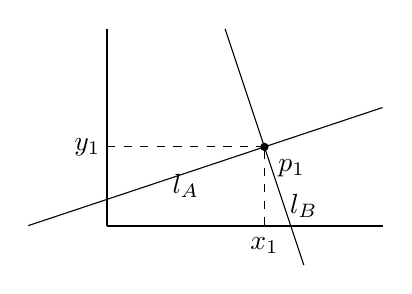
\begin{tikzpicture}[scale=0.5]
\tikzset{mark coordinate/.style={ %
		inner sep=0pt,
		outer sep=0pt,
		minimum size=3pt,
		fill=#1,
		circle %
	}
}
\draw (-2,0) -- (7,3);
\draw (5,-1) -- (3,5);
\draw[thick] (0,0) -- (7,0);
\draw[thick] (0,0) -- (0,5);

%\draw[thick] (1,1)  coordinate [mark coordinate=black,label={270:$p_0$}]   (orig);
\draw[thick] (4,2)  coordinate [mark coordinate=black,label={330:$p_1$}]   (c1);

\draw[dashed] (4,0) -- (4,2);
\draw[dashed] (0,2) -- (4,2);

\node at (2,1) {$l_A$};
\node at (5,0.5) {$l_B$};

\node at (4,-0.5) {$x_1$};
\node at (-0.5,2) {$y_1$};

\end{tikzpicture}
%\end{center}


\end{document}
